\documentclass[dv_diss_main.tex]{subfiles}





%---------------------------------------------%
%----------------Figures----------------------
%---------------------------------------------%



\newcommand{\rddplot}{
\textit{Note.}This plot aggregate data into bins of half percentage points and estimate a third order polynomial regression between the running variable and the bins on each side of the cut-off. 
}


\newcommand{\rdd}{
\textit{Note.}This table reports the estimates of political alignment from equation (2). The sample includes post electoral years of all municipalities with close elections during the period 1998-2003. The outcome variables are measure as a three year changes. Controls refers to state fixed effects, election-year fixed effects, and baseline political characteristics (incumbency status, previous political alignment, previous political party). Mean dep var refers to the sample average of the outcome variable for the non-aligned municipalities. 
}



\newcommand{\sharerev}{
Percentage of revenues is the sample average share of each source of revenue on total revenues for the non-aligned counterparts
}

\newcommand{\shareemp}{
Percentage of employment is the sample average share of each sector on total employment for the non-aligned counterparts
}

\newcommand{\event}{
\textit{Note.}The figure plots the coefficients obtained from the estimation of equation (3) discussed in Section 4. The sample includes all municipalities with close elections during the period 1998-2003. The unit of observation is  the municipal-election pair, for each pair I follow the outcome measures in [-4 +4] years window. The outcome variables are measure in inverse hyperbolic sine points. The tick(thin) lines are 90\%(95\%) confidence intervals. The specification controls by municipality-election and election-year fixed effects. 
}

%inverse hyperbolic sine (IHS) transformation


\newcommand{\stars}{
Standard errors clustered at municipality level.  *** p<0.01, ** p<0.05, * p<0.1.
}

\newcommand{\census}{
}

\newcommand{\household}{
}

%example \newcommand{\rddnote}{\figtext{\justifying{\scriptsize{Notes:                }}}}
\newcommand{\starnotes}{* denotes significance at 10 pct., ** at 5 pct., and *** at 1 pct. level.}


%---------------------------------------------%
%----------------Figures----------------------
%---------------------------------------------%

%---External validity 

\newcommand{\sammi}{
\textit{Note.}This figure presents the difference of means of baseline covariates from the 2000 population census. Each point represents the estimate of the difference in means and the line the corresponding 95 percent confidence interval. All variables are standardized. Panel A shows the difference in means between the observational sample and the OLS-weighted sample. Panel B shows the difference in means between the observational sample and the IV-weighted sample. IV model weights are estimated using a control function approach. The weights are computed  based on Aronow and Samii (2016). We include as controls time and municipality fixed effects, formula's inputs and pre-trends of all outcomes of interest.
}

\newcommand{\sammidescrip}{
	
\textit{Note.}Means and standard deviations for baseline covariates from the 2000 population census. The column of the observational sample refers to the unweighted average. The OLS and IV columns correspond to weighted averages using regression-based weights of the corresponding models. The weights of the IV model are estimated using a control function approach. The weights are computed  based on Aronow and Samii (2016). We include as controls time and municipality fixed effect, formula's inputs and pre-trends of all outcomes of interest.

}

\newcommand{\revenuebydecil}{
\textit{Note.} Calculations based on information from SIMBAD (State and Municipal System Databases), National Institute of Statistics and Geography (INEGI).
}


\newcommand{\povertylineformula}{
\textit{Note.} The Figure shows the poverty line used to compute the formula on a yearly basis. We did not include the 2001 poverty line (Mex\$1097.859) for visualization purposes. Our estimation sample includes FAIS resources allocated between 2002-2014. 

}


\newcommand{\faisvariation}{\textit{Note.} The Figure plots the distribution of the share of transfer that corresponds to each state according to the FAIS formula. The figure plots the distribution of the demeaned shares across years by state  (2002-2014). Source: State FAIS formula values are collected from the Official Federal Gazette publication made on October of every year. }
\newcommand{\pcinequality}{
\textit{Note.} Calculations using the poverty maps of 2000, 2005, 2010, and 2014. Each quantile group is approximately 112 municipalities.
}

\newcommand{\pcincomegrowth}{
\textit{Note.} numbers reported are average across municipalities. The index shows the changes in a given percentile of the  municipal household income per capita distribution. Municipalities at the nth percentile in 2000 and 2014 do not necessarily correspond.
Source: Calculations using the poverty maps of 2000, 2005, 2010, and 2014.
}

\newcommand{\figurefaistrends}{
	
\textit{Note.}Panel A plots the share of municipalities reporting to receive zero resources from FAIS. Panel B plots the average value of per-capita transfers in constant prices, normalized to be 1 in 2005. Other public revenues include taxes, debt and unconditional cash transfers

}




%---------------------------------------------%
%----------------Tables----------------------
%---------------------------------------------%

\newcommand{\maintable}{\textit{Note.}Table entries correspond to separate regressions of an outcome,  listed on the leftmost column, on the independent variable specified in the column titles. Observations are the same across specifications that are in the same column. All monetary variables (intergovernmental transfers  and household per-capita income percentiles) are in logs, coverage and poverty headcount variables are in percentage points. Standard errors (in parentheses) are clustered at the municipality level to reflect the design effect and the autocorrelation of shocks over time. 2SLS estimates report the Kleibergen-Paap rk Wald F-statistic [in brackets]. 
}


\newcommand{\indicestables}{\textit{Note.}Table entries correspond to separate regressions of an outcome,  listed on the leftmost column, on the independent variable specified in the column titles. Observations are the same across specifications that are in the same column. All the outcomes indices that aggregate the information of all the variables that belong to a specific family. The infrastructure index aggregates the information of access to electricity, connection to sewerage, access to water,
quality of floor and access to sanitation. The poverty index aggregates the information of the inverse of log of per capita income and poverty rates measured by three poverty lines (food, capabilities and assets). The inequality index aggregates the information of Gini index and all income rations considered in the main results (90/10, 50/10 and 90/50). The index of each family is a linear combination of all the variables that belong to each family where the weights are based on \cite{anderson2008multiple}. Standard errors (in parentheses) are clustered at the municipality level. All  2SLS estimates report the Kleibergen-Paap rk Wald F-statistic [in brackets].
}


\newcommand{\firststage}{
\textit{Note.} The horizontal axis scale in logs but axis labels measure in constant pesos per capita of 2014. The plotted values correspond to mean-standardized residuals from transfers on a set of controls. Each color corresponds to a different specification: i) Purple, labeled as FE, includes municipality and time fixed effects. ii) light blue, labeled as FE+ Controls, includes the same set of fixed effects and two sets of time-varying controls: a) formula inputs, b) pre-policy trends outcome trends for all our outcomes of interest. 
}


\newcommand{\firststagetable}{
	\textit{Note.} This table presents estimates from regressing observed FAIS on law-implied FAIS transfers. Standard errors (in parenthesis) are clustered at the municipality level. Panel A adds sequentially the controls of our baseline specification across columns. The other panels add on top of that other set of time-varying controls. Panel B adds over the specifications of panel A the following sociodemographic controls: proportion of the adult population by education levels (primary, secondary and tertiary), the proportion of males and the dependency ratio. Panel C adds over the specifications of panel A the following economic controls: proportion of workers by sector (agriculture, manufacturing, construction, commerce, low-skill services and high skill services) and proportion of workers by type of occupation (abstract non-routine task, routine task, manual task, and non-routine manual tasks). 
	%Panel D adds over the specifications of panel A the following political controls: the size of public sector, the share of public workers with tertiary education, local revenue sources by type(own revenue, intergovernmental transfers both earmarked and non-earmarked). 
	In column (3) we use the assets poverty rate as a reference outcome to define the control used for pre-trends; results are robust to using any other outcome of interest as reference. \\
	\starnotes
}


\newcommand{\trendsdescrip}{
	\textit{Note.} Table entries in columns (1) and (2) correspond to separate regressions of an outcome, listed on the leftmost column, and our instrument in column titles. Outcome variables were measured as annual change between 1990 and 2000s. Coefficient estimates and robust standard errors (in parenthesis) correspond to cross-sectional regressions. Column (1) shows the unconditional correlation between the pre-policy trends and our instrument. Column (2) adds the formula's inputs as controls. Column (3) shows the mean and standard deviation of the pre-policy trends, measure as the average annual difference between 2000's and 1990 values. \\
	\starnotes
}




\newcommand{\mainresults}{
Column (1) reports OLS estimates of observed FAIS on outcomes of interest.
Column (2) reports reduce form estimates of law-implied FAIS.
Column (3) to (5) reports instrumental variable estimates of observed FAIS instrumented by law-implied FAIS. Column (3) includes standard controls, Column (4) has as additional control trends of the outcome of interest for the pre-policy period (1990-2000) interacted with year dummies. Column (5) includes time varying measures of all other source of municipal revenues: taxes, unconditional transfers and other conditional transfers. \\
\starnotes
}

\newcommand{\polynomial}{
	Column (1) reports our baseline specification for comparison purposes.
	Column (2) and Column (3) reports estimates from a specification that include as controls second and third order polynomials of the formula inputs. \\
	\starnotes
	
}

\newcommand{\trend}{
	Column (1) reports our baseline specification not accounting by pre-trends. 
	Column (2) corresponds to our baseline specification, it controls by pre-trend using the annual change in the outcome of interest between 1990-2000 interacted with a year dummy.
	Column (3) controls by pre-trends using the predicted level of the outcome of interest under linear trends assumption. 
	Column (4) controls by pre-trends using the lagged value of the outcome of interest. \\
	\starnotes
}

\newcommand{\urban}{
	Column (1) reports our baseline specification applied to the entire sample. 
	Column (2) reports our baseline specification for the subsample of municipalities with more than 15,000 inhabitants. Column (3) reports our baseline specification for the subsample of municipalities with less than 15,000 inhabitants. \\
	\starnotes
}





\newcommand{\mhtnote}{
		\textit{Note.} Table entries correspond to separate regressions of an outcome, listed on the leftmost column, on the variable specified in the column title. This table  present the estimates of our preferred specification, which corresponds to estimates of column 4 in Tables~\ref{tab:3},~\ref{tab:4} and~\ref{tab:5}. Standard errors (in parentheses) are clustered at the municipality level to reflect the design effect and the autocorrelation of shocks over time. Sharpened false discovery rate (FDR) q-values following Anderson (2008) in [brackets]. Family-wise p-values based on 2,000 bootstraps of the free step-down procedure of Westfall and Young (1993) in \{curly brackets\}. All monetary variables (intergovernmental transfers and household per-capita income percentiles) are in logs, coverage and poverty headcount variables are in percentage points. 
		\\
		\starnotes using conventional inference. 
}


\newcommand{\spendingcatalog}{
\textit{Note.}Each pair of Classification and sub-classification defines an authorized line  of spending authorized by FAIS spending catalog. Type abbreviations: Direct (D), Indirect (I), Complements (C.) and Specials (S)-most commonly used for natural disasters emergencies-. Modality abbreviations: C means construction, Eq means equipment, Ex means extension, I means installation, M means maintenance, R means rehabilitation, S means substitution, pre means preschool, pri means primary school, sec means secondary school and prep means high school. Source: Lineamientos Generales para la operación del FAIS (Anexo 1), February 14, 2014 https://ww.dof.gob.mx/nota_detalle.php?codigo=5332721&fecha=14/02/2014.
}


% Regressions include but do not report the lagged dependent variable, fixed effects for randomization blocks, and a set of LASSO-selected baseline covariates, and are weighted be representative of the eligible population. Standard errors (in parentheses) are clustered at the household level to reflect the design effect. Asterices denote significance at the 10, 5, and 1 percent levels, and are based on clustered standard errors, in parentheses. Anderson (2008) sharpened q-values presented in brackets. Variables marked with a † are in inverse hyperbolic sines. Reported p-values in final two columns derived from F-tests of hypotheses that cost-benefit ratios are equal between GD Main and Large transfer amounts (GD=GDL), and between Gikuriro and GD Large (GK=GDL).




\begin{document}

\subsection{Data}

\subsubsection{Military Spending Validation}
\label{sec:app_data}

This section discusses the quality of the DoD military procurement contract microdata, and we compare them with data previously used in the literature. Figure \ref{fig:spend_comparison} compares the aggregate military spending in nominal terms at national level by fiscal years. We compare the aggregate military procurement spending derived from our microdata with the ones calculated by \cite{Nakamura2014}, \cite{Dupor2017}, and \cite{Demyanyk2019}. Overall, we conclude our data match well the trend and the level of aggregate spending used in previous works. 

\begin{figure}[ht]
    \begin{center}
       \begin{tabular}[c]{c}
    
    {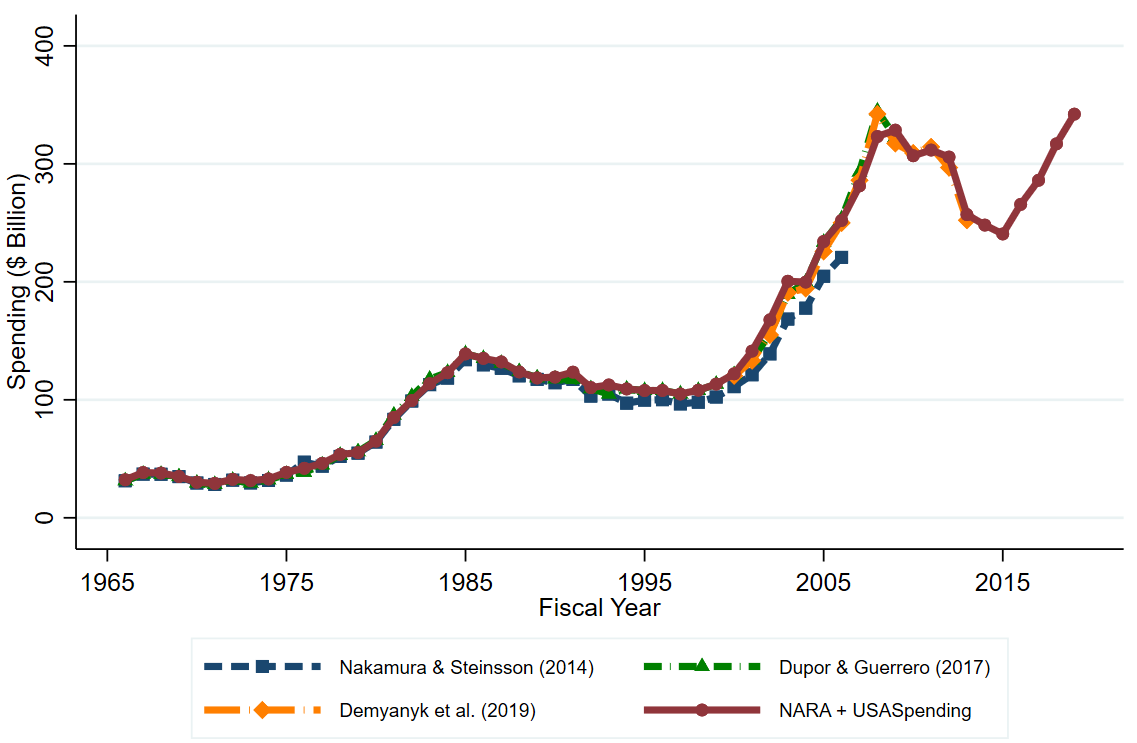
\includegraphics[height=3.5in,width=5.5in]{figures/graph_milspend_comparison.png}} \\[0.1in]

    
    \end{tabular}
    \caption{Military Spending Comparisons}\label{fig:spend_comparison}
    \end{center}
    
   
    \footnotesize{\textit{Note.} The period for the comparison matches the research design of the comparison studies. Data for the comparison studies have been downloaded from their journal's data repository.}
    
\end{figure}

As our empirical specification uses variation in military spending at local level, we also compare the level of spending at different geographically-disaggregated areas. To this end, we regress
\begin{equation*}
    Spend^{ours}_{l,t} = \beta Spend^{comp}_{l,t} + \alpha_l + \delta_{t} + \varepsilon_{l,t}
\end{equation*}
where $Spend^{ours}_{l,t}$ represents the military spending from our data in locality $l$ at time $t$; $Spend^{comp}_{l,t}$ is the spending for one of the comparison datasets; and $\alpha_l$ and $\delta_{t}$ are locality and time fixed effects, respectively.

Table \ref{tab:comp_geo} reports the results of our comparison. In column 1, we disaggregate the spending at state-level and compare our calculations with the data used by \cite{Nakamura2014}. Column 2 shows the comparison between our state-level aggregation and the ones constructed by \cite{Dupor2017}. Finally, in column 3, we show the CBSA-level comparison between our data and \cite{Demyanyk2019}.

\begin{table}[!ht]
\begin{center}
\caption{Military Spending Comparisons by Geography}
\label{tab:comp_geo}
\resizebox{0.95\linewidth}{!}{
    \begin{tabular}{l ccc} \hline 
    \vspace{-2pt} & \vspace{-2pt} & \vspace{-2pt} & \vspace{-2pt} \\
    & (1) & (2) & (3) \\
    \vspace{-2pt} & \vspace{-2pt} & \vspace{-2pt} & \vspace{-2pt} \\
    & \cite{Nakamura2014} & \cite{Dupor2017} & \cite{Demyanyk2019} \\
    \vspace{-2pt} & \vspace{-2pt} & \vspace{-2pt} & \vspace{-2pt} \\
    \cmidrule{2-4}
    & & & \\
    Military spending & 1.12 & 0.94 & 0.98 \\
    & & & \\
    $95\%$ C. I. for $\beta$ & (1.02 - 1.21) & (0.89 - 0.99) & (0.89 - 1.07) \\
    Observations & 2,050 & 2,200 & 10,636 \\
    Geographic Unit & State & State & CBSA \\
    Number Localities & 50 & 50 & 862 \\
    Period & $1966-2006$ & $1966-2009$ & $2000-2012$ \\
    Locality FE & Yes & Yes & Yes \\
    Time FE & Yes & Yes & Yes \\
     \\
    $Within-R^{2}$ & 0.97 & 0.96 & 0.79 \\
    \vspace{-2pt} & \vspace{-2pt} & \vspace{-2pt} & \vspace{-2pt} \\ \hline 

    \vspace{-2pt} & \vspace{-2pt} & \vspace{-2pt} & \vspace{-2pt} \\
\end{tabular}}
    
\end{center}
\footnotesize{\textit{Note. } The values in the brackets report the $95\%$ confidence interval. Standard errors are clustered at the geographic unit level. The period of analysis and the geographic aggregation are chosen to match the research design of the comparison studies. Data for the comparison studies have been downloaded from their journal's data repository.}
\end{table} 


We focus on two tests to evaluate the quality of the geographic distribution of our data compared to previous studies. First, as there were a one-to-one relationship between the geographic allocation between our data and previously used data, then $\beta$ should be equal or close to one. Second, if there is a strong similarity between our data and the others, then the within-$R^{2}$ should be high. The results show that the value of one is either included in the $95\%$ confidence interval or it is close the either upper or lower bound. The largest discrepancy is between our data and the ones from \cite{Nakamura2014}. This discrepancy, as showed in Figure \ref{fig:spend_comparison}, comes from the years between $2000$ and $2006$. The data collected by \cite{Nakamura2014} underestimate the aggregate spending, while ours are similar to the other sources of comparison. The within-$R^{2}$ are over $0.95$ for the comparison with \cite{Nakamura2014} and \cite{Dupor2017}, and it is a little bit lower in the comparison with \cite{Demyanyk2019}. As our data are constructed until $2006$ using NARA and USASpending after that year and \cite{Demyanyk2019} use only USASpending starting from $2001$, these tests also confirm the comparability between the information provided by NARA and USASpending. Overall, these results suggest our data are highly comparable with the ones used in previous studies.


\subsubsection{Patent Data}\label{sec:app_patentdata}

We collect patent data from PatentsView at the end of 2019. The PatentsView database contains the universe of granted patents from the US Patent and Trademark Office (USPTO) starting from 1976 until 2019. These data contain patent-level information including application dates, the type of patent, the name of the inventors, and the latitude and longitude of their addresses. We restrict our analysis to utility patents that cover the creation of a new or improved product, process, or machine. Utility patents are also commonly known as ``patents for invention,’’ and they account for about $98\%$ of the universe of patents granted by the USPTO. We also restrict to patents with application year starting from 1976. In the patent data, we do not observe the exact date in which an innovation occurs. As common in the literature, we identify the year when an innovation occurs as the application year, which is the year when the provisional application is considered complete by the USPTO, and a filing date is set. We use the latitude and longitude of the address of an inventor to geolocate the patents ans assign them to MSAs.
 
To study the effect of government spending on private innovation, we impose some additional filters to the sample. First, we remove all MSAs with incomplete histories in granted patents and citations, and with patent growth rates between two consecutive periods greater or smaller than $\pm 150\%$. Second, the truncation bias arises from the fact that patent records are only released at the grant dates when the review process by the USPTO is completed. As a result, the truncation bias causes that the number of patents in the last years of the sample are mechanically fewer. The review process takes essentially $8$ years to be fully completed.\footnote{The USPTO reports:  ``\textit{As of 12/31/2012, utility patent data, as distributed by year of application, are approximately 95\% complete for utility patent applications filed in 2004, 89\% complete for applications filed in 2005, 80\% complete for applications filed in 2006, 67\% complete for applications filed in 2007, 49\% complete for applications filed in 2008, 36\% complete for applications filed in 2009, and 19\% complete for applications filed in 2010.}’’} Thus, to alleviate the truncation bias, we end the sample period in $2011$. 

\subsubsection{List of Major Product Codes in Each Category of Spending}\label{tab:cat_list}

\\
\\
%%%%%%%%% LIST OF PRODUCT CODES %%%%%%%%%%
\noindent\textbf{Products classified as R\&D: }

AA Agriculture, AB Community Services \& Development, AC Defense Equipment, AD Defense - Other, AE & Economic Growth \& Productivity, AF Education, AG Energy, AH Environment, AJ  General Science \& Technology, AK Housing, AL Income Security, AM International Affairs \& Cooperation,
AN Medical, AP Natural Resources, AQ Social Services, AR Space, AS Transportation - Modal AT Transportation - General, AU  Transportation - Commodity, AV  Mining Activities, AZ  Other Research \& Development

\bigskip
\newline
\vspace{4}
\noindent\textbf{Products classified as Services:}

B Special Studies \& Analyses - Not R\&D, C Architect \& Engineering Services, D  Automatic Data Processing \& Telecommunication Services, E  Purchase of Structures \& Facilities, F Natural Resources \& Conservation Services, G Social Services, H Quality Control, Testing Inspection Services, J Maintenance, Repair \& Rebuilding of Equipment, K Modification of Equipment, L Technical Representative Services, M Operation of Government-Owned Facilities, N Installation of Equipment, P Salvage Services, Q  Medical Services, R Professional, Administrative \& Management Support Services, S Utilities \& Housekeeping Services, T  Photographic, Mapping, Printing \& Publication Services, U  Educational \& Training Services, V & Transportation, Travel, \& Relocation Services, W \& Lease or Rental of Equipment, X  Lease or Rental of Facilities, Y  Construction of Structures \& Facilities, Z  Maintenance, Repair or Alteration of Real Property

\newline
\bigskip
\vspace{4}
\noindent\textbf{Products classified as Goods: }

10 Weapons, 11	Nuclear Ordnance, 12	Fire Control Equipment, 13	Ammunition \& Explosives,	14	Guide Missiles		15		Aircraft \& Airframe Structural Components,	16	&	Aircraft Components \& Accessories,	17	&	Aircraft Launching, Landing \& Ground Handling Equipment	,	18	&	Space Vehicles, 19	Ships, Small Craft, Pontoons Floating Docks	20	Ships \& Marine Equipment,
22	&	Railway Equipment,
23	&	Ground Effect Vehicles, Motor Vehicles, Trailers \& Cycles;
24	Tractors;
25	Vehicular Equipment Components;
26	Tires \& Tubes
28	Engines, Turbines \& Components	
29	&	Engine Accessories
30	&	Mechanical Power Transmission Equipment
31	&	Bearings
32	&	Woodworking Machinery \& Equipment	
34	&	Metalworking Machinery	
35	&	Service \& Trade Equipment
36	&	Special Industry Machinery	
37	&	Agricultural Machinery \& Equipment	
38	&	Construction, Mining, Excavation \& Highway Maintenance Equipment	
39	&	Materials Handling Equipment
40	&	Rope, Cable, Chain \& Fittings	
41	&	Refrigeration, Air Conditionning \& Air Circulation
42	&	Fire Fighting, Rescue \& Safety Equipment	
43	&	Pumps \& Compressors
44	&	Furnace, Steam Plant \& Drying Equipment
45	&	Plumbing, Heating \& Sanitation Equipment
46	&	Water Purification \& Sewage Treatment Equipment
47	&	Pipe, Tubing, Hose \& Fittings	
48	&	Valves
49	&	Maintenance \& Repair Shop Equipment	
51	&	Hand Tools
52	&	Measuring Tools
53	&	Hardware \& Abrasives
54	&	Prefabricated Structures \& Scaffolding
55	&	Lumber, Millwork, Plywood \& Veneer	
56	&	Construction \& Building Materials
58	&	Communication, Detection \& Coherent Radiation Systems	
59	&	Electrical \& Electronic Equipment Components
60	&	Fiber Optics Materials, Components, Assemblies \& Accessories	61	&	Electric Wire \& Power Distribution Equipment
62	&	Lighting Fixtures \& Lamps	
63	&	Alarm, Signal \& Security detection Systems
65	&	Medical, Dental, \& Veterinary Equipment \& Supplies	
66	&	Instruments \& Laboratory Equipment
67	&	Photographic Equipment
68		Chemicals \& Chemical Products	
69		Training Aids \& Devices	
70		Automatic Data Processing Equipment	
71		Furniture	
72		Household \& Commercial Furnishings \& Appliances	
73		Food Preparation \& Serving Equipment	
74		Office Machines, text Processing Systems \& Visible Record Equipment	
75		Office Supplies \& Devices	
76		Books, Maps \& Other Publications	
77		Musical Instruments, Phonographs \& Home-Type Radios	
78		Recreational \& Athletic Equipment	
79		Cleaning Equipment \& Supplies	
80		Brushes, Paints, Sealers \& Adhesives	
81		Containers, Packaging \& Packing Supplies	
83		Textiles, Leather, Furs, Apparel \& Shoe	
84		Clothing, Individual Equipment \& Insignia	
85		Toiletries	
87		Agricultural Supplies	
88		Live Animals	
89		Subsistence	
91		Fuels, Lubricants, Oils \& Waxes	
93		Nonmetallic Fabricated Materials	
94		Nonmetallic Crude Materials	
95		Metal Bars, Sheets \& Shapes	
96		Ores, Minerals \& Their Primary Products	
99		Miscellaneous	 

\subsection{Additional Empirical Results}\label{sec:app_empres}

%%%%%%%%% LEVEL AND SHARE FOR MSA SAMPLE %%%%%%%%%%
Figure \ref{fig:share_comp_sample} replicates Figure \ref{fig:share_comp} only using the $326$ MSAs in the sample. Results are in line with the ones presented in the main body of the paper. There are two minor differences that we would like to pint out. First, the time series for the aggregate spending in Figure \ref{fig:share_comp_sample} is less smooth than the one that includes all contracts. This finding suggests there is between periods some spending reallocation from (or to) the MSAs in our sample to (or from) counties excluded from the analysis. In principle, as we exploit between periods geographic variation in spending, these movements from (and to) the MSAs in our sample might help in identifying the causal effects. 

\begin{figure}[ht]
    \begin{center}
        \begin{tabular}[c]{ccc}
    
    \normalsize{\bf Panel A: Aggregate Spending} & & \normalsize{\bf Panel B: Shares by Categories} \\
    {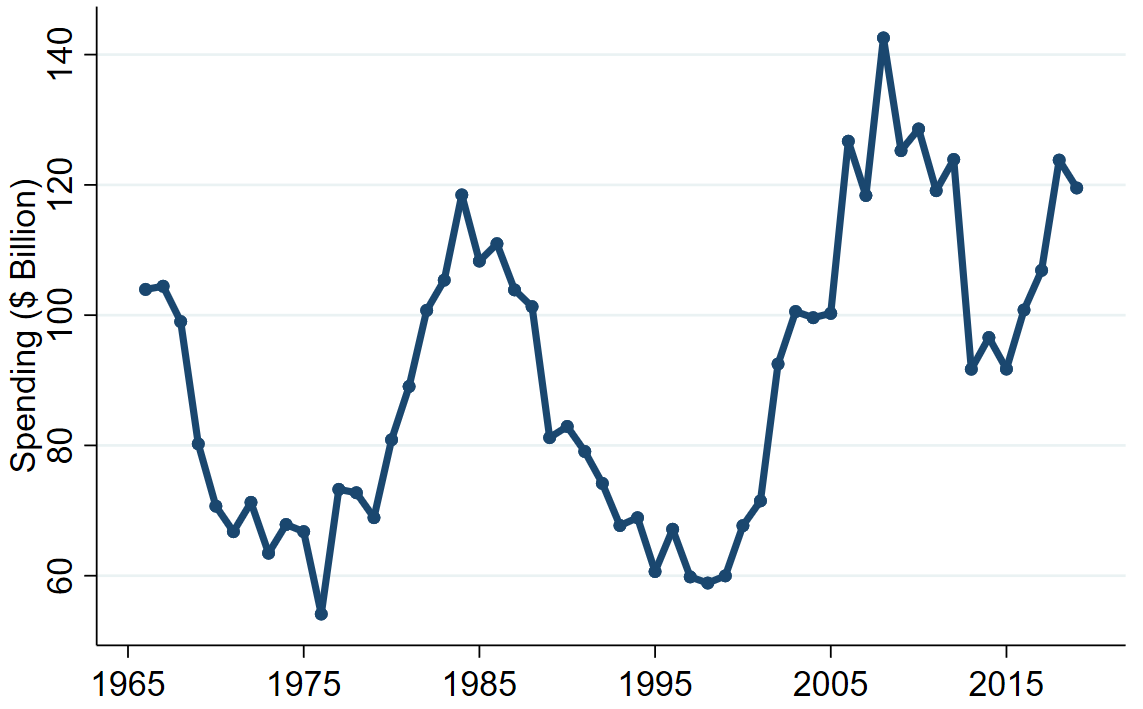
\includegraphics[height=1.8in,width=2.9in]{figures/graph_milspend_aggregate_sample.png}} & & {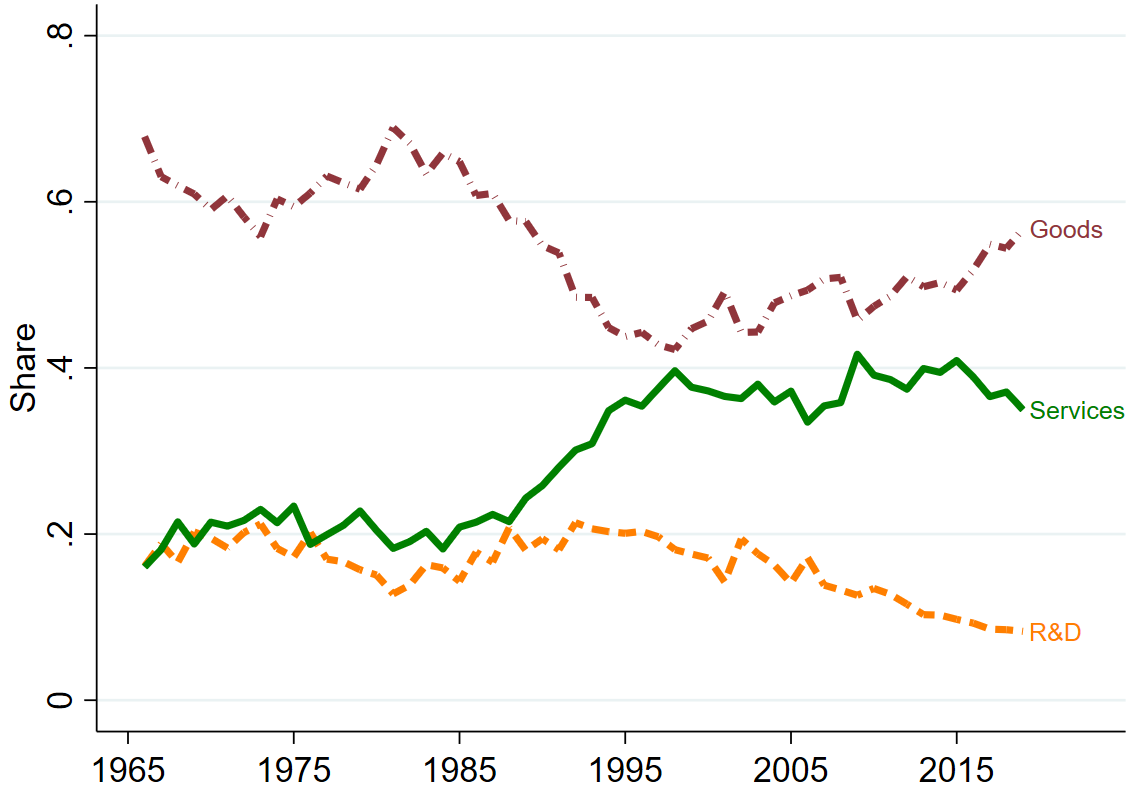
\includegraphics[height=1.8in,width=2.9in]{figures/graph_composition_shares_sample.png}} \\[0.1in]
    
    
    
    \end{tabular}
    \caption{Military Spending - Sample of Analysis}\label{fig:share_comp_sample}
    \end{center}
    
    
    \footnotesize{\textit{Note. } The national level statistics are calculated by aggregating the microdata on military procurement contracts available from NARA and USASpending.gov. Spending is in real terms by deflating the nominal value of a contract by the CPI. The classification of the spending into the three categories is based on the Federal supply classification code. The statistics are calculated by using only contracts allocated to the $296$ MSAs in our sample of analysis.}
\end{figure}

The second minor difference to highlight is that in the first couple of decades the contracts awarded to the MSAs in our sample contain a higher share of R\&D spending and a lower share of service spending than the full universe of procurement contracts.

%%%%%%%%% PER CAPITA MSA RESULTS %%%%%%%%%%
\newpage 

Table \ref{tab:fm_percapita} carries out a robustness check to the main results in which we use in the empirical specification  per capita variables at MSA-level rather than aggregate variables.

\begin{table}[H]
    \begin{center}
    \caption{Fiscal Multipliers - Earnings Per Capita}\label{tab:fm_percapita}
    \resizebox{0.95\linewidth}{!}{
    \begin{tabular}{lccccc} \hline
    \vspace{-2pt} & \vspace{-2pt} & \vspace{-2pt} & \vspace{-2pt} & \vspace{-2pt} \\
     & t & t+1 & t+2 & t+3 & t+4 \\ 
     & (1) & (2) & (3) & (4) & (5) \\
    \hline
    \vspace{-1.5pt} & \vspace{-1.5pt} & \vspace{-1.5pt} & \vspace{-1.5pt} & \vspace{-1.5pt} \\
    \multicolumn{1}{l}{\textbf{Panel A: Total Spending}} \\ 
    \vspace{-1.5pt} & \vspace{-1.5pt} & \vspace{-1.5pt} & \vspace{-1.5pt} & \vspace{-1.5pt}\\
    Military Spending & 0.382** & 0.967*** & 0.997*** & 1.208** & 1.196** \\
    & \begin{footnotesize}(0.179)\end{footnotesize} & \begin{footnotesize}(0.366)\end{footnotesize} & \begin{footnotesize}(0.365)\end{footnotesize} & \begin{footnotesize}(0.482)\end{footnotesize} & \begin{footnotesize}(0.502)\end{footnotesize} \\
    \vspace{-1.5pt} & \vspace{-1.5pt} & \vspace{-1.5pt} & \vspace{-1.5pt} & \vspace{-1.5pt} \\
    
    \multicolumn{1}{c}{\textbf{Panel B: Spending by Category}} \\ 
    \vspace{-1.5pt} & \vspace{-1.5pt} & \vspace{-1.5pt} & \vspace{-1.5pt} & \vspace{-1.5pt} \\
    R\&D Spending & 0.367 & 1.613 & 2.793 & 6.169* & 6.088* \\
    \vspace{4pt} & \begin{footnotesize}(0.472)\end{footnotesize} & \begin{footnotesize}(1.321)\end{footnotesize} & \begin{footnotesize}(1.713)\end{footnotesize} & \begin{footnotesize}(3.655)\end{footnotesize} & \begin{footnotesize}(3.447)\end{footnotesize} \\
    Services Spending & 0.748* & 1.166** & 1.259** & 1.093** & 1.247** \\
    \vspace{4pt} & \begin{footnotesize}(0.436)\end{footnotesize} & \begin{footnotesize}(0.543)\end{footnotesize} & \begin{footnotesize}(0.530)\end{footnotesize} & \begin{footnotesize}(0.526)\end{footnotesize} & \begin{footnotesize}(0.565)\end{footnotesize} \\
    Goods Spending & 0.369 & 0.645 & 0.310 & -0.511 & -0.388 \\
     & \begin{footnotesize}(0.344)\end{footnotesize} & \begin{footnotesize}(0.537)\end{footnotesize} & \begin{footnotesize}(0.496)\end{footnotesize} & \begin{footnotesize}(1.003)\end{footnotesize} & \begin{footnotesize}(0.844)\end{footnotesize} \\

    \vspace{4pt} & \begin{footnotesize}\end{footnotesize} & \begin{footnotesize}\end{footnotesize} & \begin{footnotesize}\end{footnotesize} & \begin{footnotesize}\end{footnotesize} & \begin{footnotesize}\end{footnotesize} \\
    \hline
    Observations & 10,656 & 10,656 & 10,656 & 10,656 & 10,656 \\
    Number MSA & 296 & 296 & 296 & 296 & 296 \\
    \hline
    \end{tabular}
    }
    
    \end{center}
        
    \footnotesize{\textit{Note. }Panel A reports the estimates from equation \eqref{eq:fm_base}. Panel B reports the estimates from equation \eqref{eq:fm_comp}. Standard errors are clustered at MSA level. The symbols *, **, and *** represent the $10\%$, $5\%$, and $1\%$ significance levels, respectively.}
\end{table}

%%%%%%%%% REMOVING ZEROS MSA RESULTS %%%%%%%%%%
\newpage 
Table \ref{tab:fm_restricted} reports the point estimates for a subsample of MSAs with complete histories in any spending category.

\begin{table}[H]
    \begin{center}
    \caption{Fiscal Multipliers - Removing Zero Spending in Any Category}\label{tab:fm_restricted}
    \resizebox{0.95\columnwidth}{!}{
    \begin{tabular}{lccccc} \hline
     & t & t+1 & t+2 & t+3 & t+4 \\ 
     & (1) & (2) & (3) & (4) & (5) \\
    \hline   
    & \multicolumn{5}{c}{\textbf{Dep variable: Earnings}} \\ 
    \cmidrule{2-6}
    \multicolumn{1}{l}{\textbf{Panel A: Total Spending}} \\ 
    
     Military Spending & 0.268** & 0.671*** & 0.721*** & 0.875*** & 0.798*** \\
     & \begin{footnotesize}(0.103)\end{footnotesize} & \begin{footnotesize}(0.177)\end{footnotesize} & \begin{footnotesize}(0.184)\end{footnotesize} & \begin{footnotesize}(0.224)\end{footnotesize} & \begin{footnotesize}(0.201)\end{footnotesize} \\
    
     %-------------------------------------
   
   \multicolumn{1}{l}{\textbf{Panel B: spending by category}} & & & & \\ 
    R\&D Spending & 0.279 & 0.971** & 1.594* & 1.948 & 2.286* \\
    \vspace{4pt} & \begin{footnotesize}(0.205)\end{footnotesize} & \begin{footnotesize}(0.400)\end{footnotesize} & \begin{footnotesize}(0.822)\end{footnotesize} & \begin{footnotesize}(1.245)\end{footnotesize} & \begin{footnotesize}(1.268)\end{footnotesize} \\
    Services Spending & 0.522* & 1.182*** & 1.116*** & 1.430*** & 1.348*** \\
    \vspace{4pt} & \begin{footnotesize}(0.309)\end{footnotesize} & \begin{footnotesize}(0.331)\end{footnotesize} & \begin{footnotesize}(0.420)\end{footnotesize} & \begin{footnotesize}(0.429)\end{footnotesize} & \begin{footnotesize}(0.387)\end{footnotesize} \\
    Goods Spending & 0.060 & 0.154 & 0.088 & 0.122 & 0.068 \\
     & \begin{footnotesize}(0.117)\end{footnotesize} & \begin{footnotesize}(0.217)\end{footnotesize} & \begin{footnotesize}(0.261)\end{footnotesize} & \begin{footnotesize}(0.380)\end{footnotesize} & \begin{footnotesize}(0.325)\end{footnotesize} \\
     \vspace{-2pt} & \vspace{-2pt} & \vspace{-2pt} & \vspace{-2pt} & \vspace{-2pt} \\
     \hline 
     & \multicolumn{5}{c}{\textbf{Dep variable: Employment}} \\ 
    \cmidrule{2-6}
    
     \multicolumn{1}{l}{\textbf{Panel C: Total Spending}} \\ 
    Military Spending & 0.127** & 0.297*** & 0.321*** & 0.380*** & 0.343*** \\
     & \begin{footnotesize}(0.052)\end{footnotesize} & \begin{footnotesize}(0.086)\end{footnotesize} & \begin{footnotesize}(0.096)\end{footnotesize} & \begin{footnotesize}(0.115)\end{footnotesize} & \begin{footnotesize}(0.102)\end{footnotesize} \\
    \vspace{-1.5pt} & \vspace{-1.5pt} & \vspace{-1.5pt} & \vspace{-1.5pt} & \vspace{-1.5pt} \\
    
    \multicolumn{1}{l}{\textbf{Panel D: spending by category}} & & & & \\ 
   R\&D Spending & 0.285** & 0.516** & 0.879** & 1.124* & 1.235** \\
    \vspace{4pt} & \begin{footnotesize}(0.142)\end{footnotesize} & \begin{footnotesize}(0.199)\end{footnotesize} & \begin{footnotesize}(0.420)\end{footnotesize} & \begin{footnotesize}(0.572)\end{footnotesize} & \begin{footnotesize}(0.621)\end{footnotesize} \\
    Services Spending & 0.042 & 0.348** & 0.339* & 0.454** & 0.383* \\
    \vspace{4pt} & \begin{footnotesize}(0.120)\end{footnotesize} & \begin{footnotesize}(0.165)\end{footnotesize} & \begin{footnotesize}(0.185)\end{footnotesize} & \begin{footnotesize}(0.196)\end{footnotesize} & \begin{footnotesize}(0.199)\end{footnotesize} \\
    Goods Spending & 0.080 & 0.152 & 0.097 & 0.110 & 0.103 \\
     & \begin{footnotesize}(0.066)\end{footnotesize} & \begin{footnotesize}(0.124)\end{footnotesize} & \begin{footnotesize}(0.149)\end{footnotesize} & \begin{footnotesize}(0.210)\end{footnotesize} & \begin{footnotesize}(0.182)\end{footnotesize} \\

    \vspace{4pt} & \begin{footnotesize}\end{footnotesize} & \begin{footnotesize}\end{footnotesize} & \begin{footnotesize}\end{footnotesize} & \begin{footnotesize}\end{footnotesize} & \begin{footnotesize}\end{footnotesize} \\
    \hline
    Observations & 4,068 & 4,068 & 4,068 & 4,068 & 4,068 \\
    \vspace{-2pt} & \vspace{-2pt} & \vspace{-2pt} & \vspace{-2pt} & \vspace{-2pt} \\
    Number MSA & 113 & 113 & 113 & 113 & 113 \\
    \vspace{-2pt} & \vspace{-2pt} & \vspace{-2pt} & \vspace{-2pt} & \vspace{-2pt} \\
    \hline
    
    \end{tabular}
    }
    
    \end{center}
       
    \footnotesize{\textit{Note. }Panel A reports the estimates from equation \eqref{eq:fm_base}. Panel B reports the estimates from equation \eqref{eq:fm_comp}. Standard errors are clustered at MSA level. The symbols *, **, and *** represent the $10\%$, $5\%$, and $1\%$ significance levels, respectively.}
\end{table}

\newpage
Table \ref{tab:fm_main_cum} reports the point estimates whn both the outcome and spending variable are defined as the cumulative sum of spending as indicated below 
\begin{table}[H]
    \begin{center}
    
    \caption{Estimates of Employment and Earnings Multipliers - Cumulative Specification}\label{tab:fm_main_cum}

	\resizebox*{0.95\textwidth}{!}	{
    
    \begin{tabular}{lccccc} \hline
    \vspace{-2pt} & \vspace{-2pt} & \vspace{-2pt} & \vspace{-2pt} & \vspace{-2pt} \\
     & t & t+1 & t+2 & t+3 & t+4 \\ 
     & (1) & (2) & (3) & (4) & (5) \\
    \hline
    %\cmidrule{1-6}
    \vspace{-1.5pt} & \vspace{-1.5pt} & \vspace{-1.5pt} & \vspace{-1.5pt} & \vspace{-1.5pt} \\
    &\multicolumn{5}{c}{\textbf{Dep Variable: Earnings}} \\ 
    \cmidrule{2-6}
      &  &  &  &  \\
   
   %-------------------------------------
    
   
    \multicolumn{1}{l}{\textbf{Panel A: Aggregate spending}} & & & & \\
    %\cmidrule{2-6}
    Military Spending & 0.212*** & 0.446*** & 0.529*** & 0.603*** & 0.619*** \\
    & \begin{footnotesize}(0.074)\end{footnotesize} & \begin{footnotesize}(0.133) \end{footnotesize} & \begin{footnotesize}(0.156)\end{footnotesize} & \begin{footnotesize}(0.178)\end{footnotesize} & \begin{footnotesize}(0.180)\end{footnotesize} \\
    %\cmidrule{2-6}
    
    %-------------------------------------
   \multicolumn{1}{l}{\textbf{Panel B: spending by category}} & & & & \\ 
    %\cmidrule{2-6}
   
    R\&D Spending & 0.305* & 1.020** & 1.681** & 2.337** & 2.614** \\
     & \begin{footnotesize}(0.179)\end{footnotesize} & \begin{footnotesize}(0.384)\end{footnotesize} & \begin{footnotesize}(0.646)\end{footnotesize} & \begin{footnotesize}(0.914)\end{footnotesize} & \begin{footnotesize}(1.019)\end{footnotesize} \\

      
    Services Spending & 0.345*** & 0.597*** &         0.683*** &         0.784***   &       0.813*** \\
     & \begin{footnotesize}(0.101)\end{footnotesize} & \begin{footnotesize}(0.154)\end{footnotesize} & \begin{footnotesize}(0.161)\end{footnotesize} & \begin{footnotesize}(0.177)\end{footnotesize} & \begin{footnotesize}(0.178)\end{footnotesize} \\

    Goods Spending & 0.097 & 0.108 & 0.0373 & -0.0166 & -0.0289 \\
     & \begin{footnotesize}(0.079)\end{footnotesize} & \begin{footnotesize}(0.126)\end{footnotesize} & \begin{footnotesize}(0.136)\end{footnotesize} & \begin{footnotesize}(0.161)\end{footnotesize} & \begin{footnotesize}(0.169)\end{footnotesize} \\
  % \\
  % Test $\beta^k_g=\beta^k_s=\beta^k_{rd}$  &  [0.1360]  & [0.0113] & [0.0029] & [0.0038] & [0.0025] \\
  % \\
    \hline
    \vspace{-2pt} & \vspace{-2pt} & \vspace{-2pt} & \vspace{-2pt} & \vspace{-2pt} \\
    & \multicolumn{5}{c}{\textit{\textbf{Dep Variable: : Employment}}} \\ 
    \cmidrule{2-6}
    
    %-------------------------------------
   \multicolumn{1}{l}{\textbf{Panel C: Aggregate spending}} & & & & \\

    Military Spending & 0.131*** &  0.250*** & 0.297*** & 0.333*** & 0.340*** \\
    & \begin{footnotesize}(0.043)\end{footnotesize} & \begin{footnotesize}(0.071)\end{footnotesize} & \begin{footnotesize}(0.086)\end{footnotesize} & \begin{footnotesize}(0.098)\end{footnotesize} & \begin{footnotesize}(0.099)\end{footnotesize} \\
    
    %-------------------------------------
     \multicolumn{1}{l}{\textbf{Panel D: spending by category}} & & & & \\
    R\&D Spending & 0.167* & 0.451** & 0.793** &  1.113** & 1.241**  \\
    \vspace{4pt} & \begin{footnotesize}(0.101)\end{footnotesize} & \begin{footnotesize}(0.176) \end{footnotesize} & \begin{footnotesize}(0.299)\end{footnotesize} & \begin{footnotesize}(0.403)\end{footnotesize} & \begin{footnotesize}(0.454)\end{footnotesize} \\
    
    Services Spending & 0.190*** &  0.309*** &  0.361*** & 0.409*** & 0.407*** \\
    \vspace{4pt} & \begin{footnotesize}(0.036)\end{footnotesize} & \begin{footnotesize} (0.057) \end{footnotesize} & \begin{footnotesize}(0.057) \end{footnotesize} & \begin{footnotesize}(0.060)\end{footnotesize} & \begin{footnotesize}(0.059)\end{footnotesize} \\
   

    Goods Spending & 0.080 & 0.0919  & 0.0520 & 0.0312 & 0.0338 \\
    & \begin{footnotesize}(0.051)\end{footnotesize} & \begin{footnotesize}(0.081)\end{footnotesize} & \begin{footnotesize} (0.083)\end{footnotesize} & \begin{footnotesize}(0.093)\end{footnotesize} & \begin{footnotesize}(0.098)\end{footnotesize} \\
   
   % \\
    %Test $\beta^k_g=\beta^k_s=\beta^k_{rd}$  &  [0.218]  & [0.0563] & [0.0012] & [0.0017] & [0.0078] \\
   %\\
    \hline
    \vspace{-2pt} &  & & & & \\ 
    Observations & 10,656 & 10,656 & 10,656 & 10,656 & 10,656 \\
    Number MSA & 296 & 296 & 296 & 296 & 296 \\
    \hline \hline \\
    \vspace{-2pt} & \vspace{-2pt} & \vspace{-2pt} & \vspace{-2pt} \\
    \end{tabular}

    %Notes: Estimation sample for all specifications includes data from 1980-2015, with Observations=10656 and MSA=296. This table reports the estimates of cumulative earnings and employment multipliers as defined by \cite{ramey2018government}. The difference with main specification is that the outcomes variables are defined as the cumulative change between period $t-1$ and $t+k$, as follows: $\sum_{k}(\frac{v_{l,t+k}-v_{l,t-1}}{v_{l,t-1}})$. Similarly spending (aggregate or for each category) is defined as $\sum_{k}(\frac{G_{l,t+k}-G_{l,t-1}}{Y_{l,t-1}})$. Panel A and C reports the IV estimates from equation \eqref{eq:fm_base}. Panel B and D reports the IV estimates from equation \eqref{eq:fm_comp}. Both specifications include MSA and time fixed effects.  Standard errors are clustered at MSA level. The symbols *, **, and *** represent the $10\%$, $5\%$, and $1\%$ significance levels, respectively.}
    
   
    }
    \end{center}
    \footnotesize {
    \textit{Note. } Estimation sample for all specifications includes data from 1980-2015, with Observations=10656 and MSA=296. This table reports the estimates of cumulative earnings and employment multipliers as defined by \cite{ramey2018government}. The difference with main specification is that the outcomes variables are defined as the cumulative change between period $t-1$ and $t+k$, as follows: $\sum_{k}(\frac{v_{l,t+k}-v_{l,t-1}}{v_{l,t-1}})$. Similarly spending (aggregate or for each category) is defined as $\sum_{k}(\frac{G_{l,t+k}-G_{l,t-1}}{Y_{l,t-1}})$. Panel A and C reports the IV estimates from equation \eqref{eq:fm_base}. Panel B and D reports the IV estimates from equation \eqref{eq:fm_comp}. Both specifications include MSA and time fixed effects.  Standard errors are clustered at MSA level. The symbols *, **, and *** represent the $10\%$, $5\%$, and $1\%$ significance levels, respectively.}

\end{table}
\newpage

%%%%%%%%%%%%%%%%5 INDUSTRY CLASSIFICATION ISSUE %%%%%%%%%%%%%

%
%
%
%
%%%%%%%%%%%%%% INDUSTRY CLASSIFICATION %%%%%%%%%%%%%%%%%
\newpage
\begin{table}[H]
\begin{center}
\caption{Industry Classification by Labor Intensity}
\label{tab:indlabint_list}
\resizebox{0.7\textwidth}{0.46\textheight}{
\begin{tabular}{ccc} \hline
\vspace{-3pt} & \vspace{-3pt} \\
& NAICS Code & Sector \\ 
\vspace{-3pt} & \vspace{-3pt} \\ \hline
\vspace{-3pt} & \vspace{-3pt} \\
\multirow{30}{*}{\makecell{Low \\Labor \\Intensity}} & 111-112 & Farms \\
& 113-115 & Forestry, fishing, and related activities \\ 
& 211 & Oil and gas extraction \\ 
& 212 & Mining, except oil and gas \\ 
& 22 & Utilities \\
& 311-312 & Food and beverage and tobacco products \\ 
& 322 & Paper products \\
& 324 & Petroleum and coal products \\ 
& 325 & Chemical products \\ 
& 327 & Nonmetallic mineral products \\ 
& 331 & Primary metals \\ 
& 334 & Computer and electronic products \\ 
& 3361-3363 & Motor vehicles, bodies and trailers, and parts \\
& 42 & Wholesale trade \\ 
& 44-45 & Retail trade \\ 
& 481 & Air transportation \\ 
& 483 & Water transportation \\ 
& 485 & Transit and ground passenger transportation \\ 
& 486 & Pipeline transportation \\
& 512 & Motion picture and sound recording industries \\ 
& 515; 517 & Broadcasting and telecommunications \\
& 521-522 & Federal Reserve banks, credit intermediation, and related activities \\ 
& 524 & Insurance carriers and related activities \\
& 525 & Funds, trusts, and other financial vehicles \\ 
& 531 & Real estate \\ \
& 532-533 & Rental and leasing services and lessors of intangible assets \\
& 5411 & Legal services \\
& 562 & Waste management and remediation services \\
& 711-712 & Performing arts, spectator sports, museums, and related activities \\ 
& 721 & Accommodation \\ 
\vspace{-3pt} & \vspace{-3pt} \\ \hline
\vspace{-3pt} & \vspace{-3pt} \\
\multirow{28}{*}{\makecell{High \\Labor \\Intensity}} & 213 & Support activities for mining \\
& 23 & Construction \\ 
& 313-314 & Textile mills and textile product mills \\ 
& 315-316 & Apparel and leather and allied products \\ 
& 321 & Wood products \\
& 323 & Printing and related support activities \\ 
& 326 & Plastics and rubber products \\ 
& 332 & Fabricated metal products \\ 
& 333 & Machinery \\
& 335 & Electrical equipment, appliances, and components \\ 
& 3364-3366; 3369 & Other transportation equipment \\ 
& 337 & Furniture and related products \\ 
& 339 & Miscellaneous manufacturing \\ 
& 482 & Rail transportation \\ 
& 484 & Truck transportation \\ 
& 487-488; 492 & Other transportation and support activities \\ 
& 493 & Warehousing and storage \\ 
& 523 & Securities, commodity contracts, and investments \\
& 5412-5414; 5416-5419 & Miscellaneous professional, scientific, and technical services \\
& 5415 & Computer systems design and related services \\ 
& 55 & Management of companies and enterprises \\ 
& 561 & Administrative and support services \\ 
& 61 & Educational services \\
& 621 & Ambulatory health care services \\ 
& 624 & Social assistance \\ 
& 713 & Amusements, gambling, and recreation industries \\ 
& 722 & Food services and drinking places \\
& 81 & Other services, except government \\ 
\vspace{-3pt} & \vspace{-3pt} \\ \hline
\end{tabular}
}
\end{center}
\end{table}





%%%%%%%%% STATE RESULTS %%%%%%%%%%
\newpage 
Table \ref{tab:fm_state} reports the point estimates computed by aggregating military spending at state-level rather than MSA-level.
\begin{table}[H]
    \begin{center}
    \caption{Fiscal Multipliers - State Aggregation} \label{tab:fm_state}
    \resizebox{0.95\linewidth}{!}{
    \begin{tabular}{lccccc} \hline
    \vspace{-2pt} & \vspace{-2pt} & \vspace{-2pt} & \vspace{-2pt} & \vspace{-2pt} \\
     & t & t+1 & t+2 & t+3 & t+4 \\ 
     & (1) & (2) & (3) & (4) & (5) \\
    \hline   
    & \multicolumn{5}{c}{\textbf{Dep variable: Earnings}} \\ 
    \cmidrule{2-6}
    \multicolumn{6}{l}{\textbf{Panel A: Total Spending}} \\ 
     Military Spending & 0.449* & 1.341** & 1.294** & 1.813** & 1.544** \\
    & \begin{footnotesize}(0.253)\end{footnotesize} & \begin{footnotesize}(0.601)\end{footnotesize} & \begin{footnotesize}(0.575)\end{footnotesize} & \begin{footnotesize}(0.730)\end{footnotesize} & \begin{footnotesize}(0.642)\end{footnotesize} \\
    
    \multicolumn{6}{l}{\textbf{Panel B: Spending by Category}} \\ 
    
    R\&D Spending & -0.708 & 3.812 & 5.380 & 9.514 & 9.784* \\
    \vspace{4pt} & \begin{footnotesize}(1.594)\end{footnotesize} & \begin{footnotesize}(3.642)\end{footnotesize} & \begin{footnotesize}(4.569)\end{footnotesize} & \begin{footnotesize}(6.146)\end{footnotesize} & \begin{footnotesize}(5.361)\end{footnotesize} \\
    Services Spending & 4.567* & 6.475* & 5.030* & 4.621* & 4.380* \\
    \vspace{4pt} & \begin{footnotesize}(2.559)\end{footnotesize} & \begin{footnotesize}(3.811)\end{footnotesize} & \begin{footnotesize}(2.508)\end{footnotesize} & \begin{footnotesize}(2.682)\end{footnotesize} & \begin{footnotesize}(2.497)\end{footnotesize} \\
    Goods Spending & 0.024 & -0.381 & -0.645 & -0.997 & -1.133 \\
     & \begin{footnotesize}(0.293)\end{footnotesize} & \begin{footnotesize}(0.699)\end{footnotesize} & \begin{footnotesize}(0.899)\end{footnotesize} & \begin{footnotesize}(1.075)\end{footnotesize} & \begin{footnotesize}(1.016)\end{footnotesize} \\

     \hline
    \vspace{-2pt} & \vspace{-2pt} & \vspace{-2pt} & \vspace{-2pt} & \vspace{-2pt} \\
    
    & \multicolumn{5}{c}{\textbf{Dep variable: Employment}} \\
    \cmidrule{2-6}
    \multicolumn{6}{l}{\textbf{Panel C: Total Spending}} \\ 
     Military Spending & 0.219** & 0.723** & 0.826** & 1.168** & 1.065** \\
     & \begin{footnotesize}(0.108)\end{footnotesize} & \begin{footnotesize}(0.355)\end{footnotesize} & \begin{footnotesize}(0.332)\end{footnotesize} & \begin{footnotesize}(0.472)\end{footnotesize} & \begin{footnotesize}(0.415)\end{footnotesize} \\
    
    \multicolumn{1}{l}{\textbf{Panel D: Spending by Category}} \\ 
    R\&D Spending & 0.465 & 2.086* & 2.883** & 5.294** & 5.049** \\
    \vspace{4pt} & \begin{footnotesize}(0.379)\end{footnotesize} & \begin{footnotesize}(1.094)\end{footnotesize} & \begin{footnotesize}(1.418)\end{footnotesize} & \begin{footnotesize}(2.124)\end{footnotesize} & \begin{footnotesize}(2.110)\end{footnotesize} \\
    Services Spending & 1.205** & 1.638* & 1.523 & 1.082 & 0.895 \\
    \vspace{4pt} & \begin{footnotesize}(0.569)\end{footnotesize} & \begin{footnotesize}(0.874)\end{footnotesize} & \begin{footnotesize}(1.035)\end{footnotesize} & \begin{footnotesize}(1.140)\end{footnotesize} & \begin{footnotesize}(1.133)\end{footnotesize} \\
    Goods Spending & 0.060 & 0.260 & 0.222 & 0.308 & 0.367 \\
     & \begin{footnotesize}(0.155)\end{footnotesize} & \begin{footnotesize}(0.371)\end{footnotesize} & \begin{footnotesize}(0.457)\end{footnotesize} & \begin{footnotesize}(0.667)\end{footnotesize} & \begin{footnotesize}(0.715)\end{footnotesize} \\


    \vspace{4pt} & \begin{footnotesize}\end{footnotesize} & \begin{footnotesize}\end{footnotesize} & \begin{footnotesize}\end{footnotesize} & \begin{footnotesize}\end{footnotesize} & \begin{footnotesize}\end{footnotesize} \\
    \hline
    Observations & 1,836 & 1,836 & 1,836 & 1,836 & 1,836 \\
    Number State & 51 & 51 & 51 & 51 & 51 \\
   \hline

    \end{tabular}
    }
   
    \end{center}
        
    \footnotesize{\textit{Note. }Panel A reports the estimates from equation \eqref{eq:fm_base}. Panel B reports the estimates from equation \eqref{eq:fm_comp}. Standard errors are clustered at state level. The symbols *, **, and *** represent the $10\%$, $5\%$, and $1\%$ significance levels, respectively.}
\end{table}

\newpage 
Table \ref{tab:earn_spill} reports the point estimates of the effects of local government spending on earnings in the neighboring locations.
\begin{table}[H]

    \begin{center}
    \caption{Fiscal Multiplier in the Neighboring Locations - Earnings}\label{tab:earn_spill}
    
    
    \resizebox{0.95\linewidth}{!}{
    \begin{tabular}{lccccc} \hline
    \vspace{-2pt} & \vspace{-2pt} & \vspace{-2pt} & \vspace{-2pt} & \vspace{-2pt} \\
     & t & t+1 & t+2 & t+3 & t+4 \\ 
     & (1) & (2) & (3) & (4) & (5) \\
    
    \hline
    \multicolumn{1}{l}{\textbf{Panel A: Total Spending}} \\ 
    
    \vspace{-1.5pt} & \vspace{-1.5pt} & \vspace{-1.5pt} & \vspace{-1.5pt} & \vspace{-1.5pt}\\
    Military Spending & 0.010 & 0.002 & 0.003 & 0.007 & 0.014 \\
    & \begin{footnotesize}(0.009)\end{footnotesize} & \begin{footnotesize}(0.012)\end{footnotesize} & \begin{footnotesize}(0.012)\end{footnotesize} & \begin{footnotesize}(0.012)\end{footnotesize} & \begin{footnotesize}(0.014)\end{footnotesize} \\
    \vspace{-1.5pt} & \vspace{-1.5pt} & \vspace{-1.5pt} & \vspace{-1.5pt} & \vspace{-1.5pt} \\
    
    \multicolumn{1}{c}{\textbf{Panel B: Spending by Category}} \\ 
    
    R\&D Spending & -0.052** & -0.246 & -0.536* & -1.023 & -0.357 \\
    \vspace{4pt} & \begin{footnotesize}(0.023)\end{footnotesize} & \begin{footnotesize}(0.243)\end{footnotesize} & \begin{footnotesize}(0.280)\end{footnotesize} & \begin{footnotesize}(0.671)\end{footnotesize} & \begin{footnotesize}(0.350)\end{footnotesize} \\
    Services Spending & 0.037*** & 0.054*** & 0.110* & 0.283 & 0.146 \\
    \vspace{4pt} & \begin{footnotesize}(0.007)\end{footnotesize} & \begin{footnotesize}(0.015)\end{footnotesize} & \begin{footnotesize}(0.057)\end{footnotesize} & \begin{footnotesize}(0.195)\end{footnotesize} & \begin{footnotesize}(0.147)\end{footnotesize} \\
    Goods Spending & 0.019 & 0.044 & 0.082 & 0.103 & 0.037 \\
     & \begin{footnotesize}(0.030)\end{footnotesize} & \begin{footnotesize}(0.096)\end{footnotesize} & \begin{footnotesize}(0.094)\end{footnotesize} & \begin{footnotesize}(0.074)\end{footnotesize} & \begin{footnotesize}(0.056)\end{footnotesize} \\

    \vspace{4pt} & \begin{footnotesize}\end{footnotesize} & \begin{footnotesize}\end{footnotesize} & \begin{footnotesize}\end{footnotesize} & \begin{footnotesize}\end{footnotesize} & \begin{footnotesize}\end{footnotesize} \\
    Observations & 10,224 & 10,224 & 10,224 & 10,224 & 10,224 \\
    Number MSA & 284 & 284 & 284 & 284 & 284 \\
    \hline
    \end{tabular}
    }
    
    \end{center}
       
    \footnotesize{\textit{Note. }Estimates are computed from  equation \eqref{eq:fm_spill}. The unit of observations are MSAs in different years. Standard errors are clustered at MSA level. The symbols *, **, and *** represent the $10\%$, $5\%$, and $1\%$ significance levels, respectively.}

\end{table}

%%%%%%%%%% PRIVATE CONSUMPTION EXPENDITURE %%%%%%%%%%%%%%
\newpage
Table \ref{tab:crowd_privcons} reports the crowding out effect of government spending on private consumption expenditure.

\begin{table}[H]
    \begin{center}
    \caption{Private Consumption Expenditure Crowding-out Effect}\label{tab:crowd_privcons}
    \resizebox{0.95\linewidth}{!}{
    \begin{tabular}{lccccc} \hline
    \vspace{-2pt} & \vspace{-2pt} & \vspace{-2pt} & \vspace{-2pt} & \vspace{-2pt} \\
     & t & t+1 & t+2 & t+3 & t+4 \\ 
     & (1) & (2) & (3) & (4) & (5) \\
    
    \hline
    \multicolumn{1}{l}{\textbf{Panel A: Total Spending}} \\ 
    Military Spending & 0.071 & 0.054 & -0.013 & -0.169 & -0.192 \\
    & \begin{footnotesize}(0.067)\end{footnotesize} & \begin{footnotesize}(0.229)\end{footnotesize} & \begin{footnotesize}(0.299)\end{footnotesize} & \begin{footnotesize}(0.526)\end{footnotesize} & \begin{footnotesize}(0.505)\end{footnotesize} \\
    \vspace{-1.5pt} & \vspace{-1.5pt} & \vspace{-1.5pt} & \vspace{-1.5pt} & \vspace{-1.5pt} \\
    
    \multicolumn{1}{c}{\textbf{Panel B: Spending by Category}} \\ 
    R\&D Spending & -0.591 & -0.208 & 0.435 & 0.365 & 0.820 \\
    \vspace{4pt} & \begin{footnotesize}(1.061)\end{footnotesize} & \begin{footnotesize}(1.185)\end{footnotesize} & \begin{footnotesize}(2.178)\end{footnotesize} & \begin{footnotesize}(2.107)\end{footnotesize} & \begin{footnotesize}(2.273)\end{footnotesize} \\
    Services Spending & 0.624 & 0.504 & -0.049 & -0.261 & -0.373 \\
    \vspace{4pt} & \begin{footnotesize}(0.747)\end{footnotesize} & \begin{footnotesize}(1.119)\end{footnotesize} & \begin{footnotesize}(1.637)\end{footnotesize} & \begin{footnotesize}(1.572)\end{footnotesize} & \begin{footnotesize}(1.694)\end{footnotesize} \\
    Goods Spending & 0.088 & -0.056 & -0.164 & -0.328 & -0.493 \\
     & \begin{footnotesize}(0.164)\end{footnotesize} & \begin{footnotesize}(0.281)\end{footnotesize} & \begin{footnotesize}(0.558)\end{footnotesize} & \begin{footnotesize}(0.868)\end{footnotesize} & \begin{footnotesize}(0.851)\end{footnotesize} \\

    \vspace{4pt} & \begin{footnotesize}\end{footnotesize} & \begin{footnotesize}\end{footnotesize} & \begin{footnotesize}\end{footnotesize} & \begin{footnotesize}\end{footnotesize} & \begin{footnotesize}\end{footnotesize} \\
    Observations & 918 & 918 & 918 & 918 & 918 \\
    Number State & 51 & 51 & 51 & 51 & 51 \\
     \hline
     \\
    \end{tabular}
    }
    
    \end{center}
    \footnotesize{\textit{Note. }Standard errors are clustered at state-level. The symbols *, **, and *** represent the $10\%$, $5\%$, and $1\%$ significance levels, respectively.}
\end{table}

\end{document}